	\subsection{PSF Intensities clustering}

		\subsubsection{K-Means}
			
			As K-Means allows for the number of clusters to be defined, and we know that there are 4 in the original dataset, K-Means is used to find 4 clusters.
			
			\begin{table}[h!]
				\centering
				\begin{tabular}{|c|c|c|}
					\hline
					& \textbf{Number of clusters} & \textbf{Number of initializations}\\
					\hline
					\textbf{PCA PSF Intensities} & 4 & 10\\
					\hline
					\textbf{UMAP PSF Intensities} & 4 & 10\\
					\hline
				\end{tabular}
				\caption{K-Means hyperparameter configuration for c coefficients clustering}
			\end{table}
		
			\begin{figure*}[ht!]
				\centering
				\subfloat[Original cluster densities from PCA]{%
					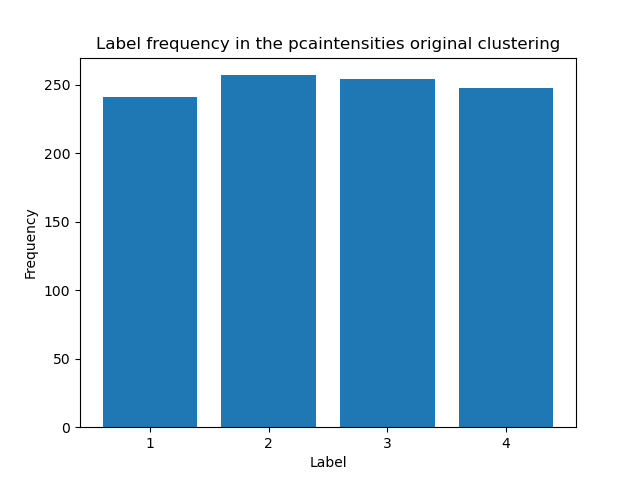
\includegraphics[width=0.45\textwidth]{mdid-pcaintensitiesoriginaldensity.png}}
				\hspace{\fill}
				\subfloat[K-Means clusters densities from PCA]{%
					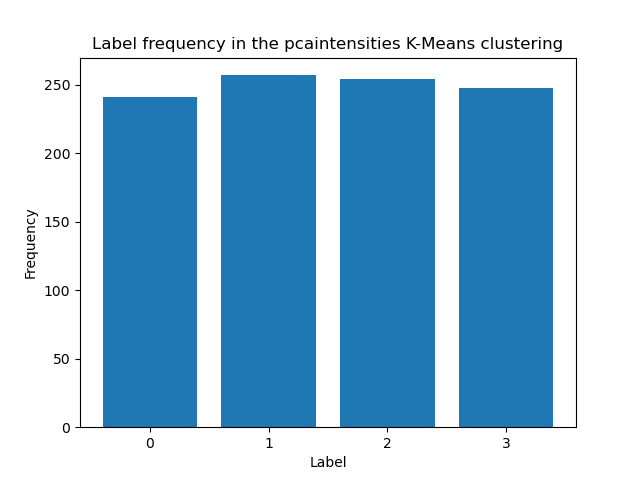
\includegraphics[width=0.45\textwidth]{mdid-pcaintensitiesK-Meansdensity.png}}\\
				\subfloat[Original clusters]{%
					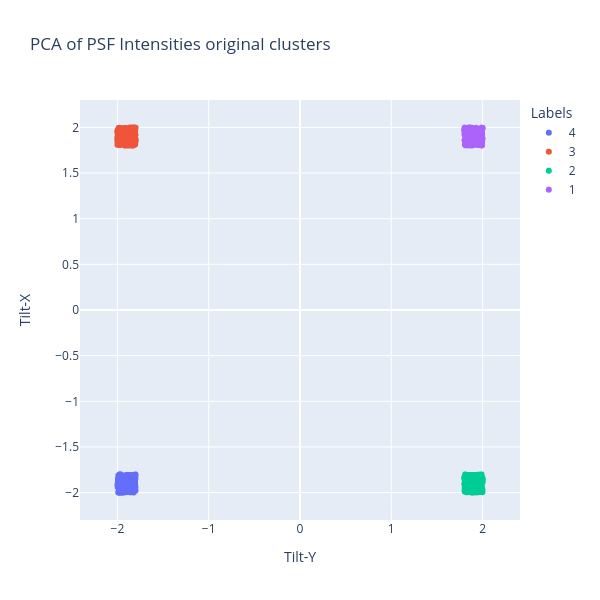
\includegraphics[width=0.45\textwidth]{mdid-pcaintensitiesoriginalclusters.png}}
				\hspace{\fill}
				\subfloat[K-Means clusters from PCA]{%
					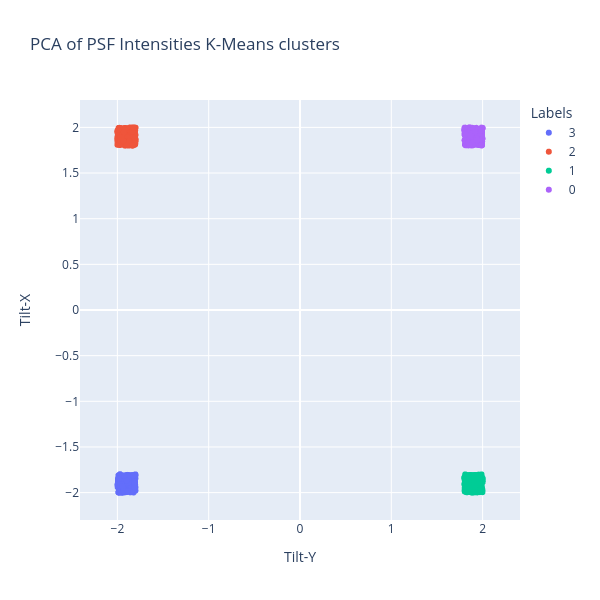
\includegraphics[width=0.45\textwidth]{mdid-pcaintensitiesK-Meansclusters.png}}\\
					
				\subfloat[Original cluster samples from PCA]{%
					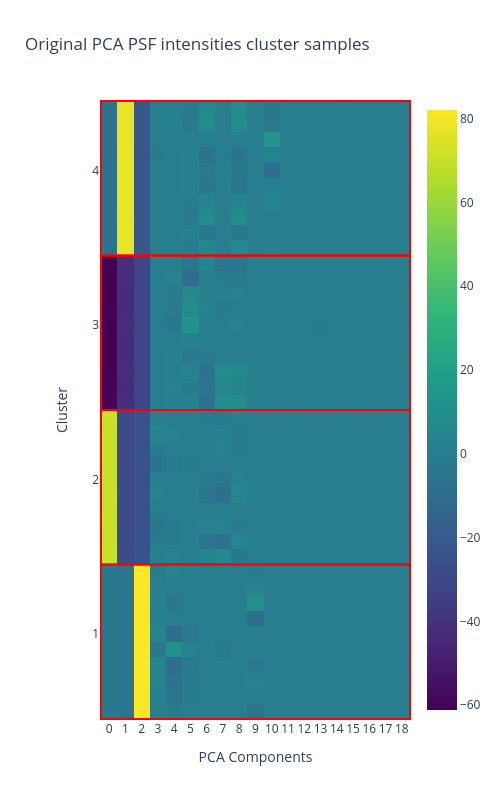
\includegraphics[width=0.4\textwidth]{mdid-pcaintensitiesoriginalgridclusters.png}}
				\hspace{\fill}
				\subfloat[K-Means cluster samples from PCA]{%
					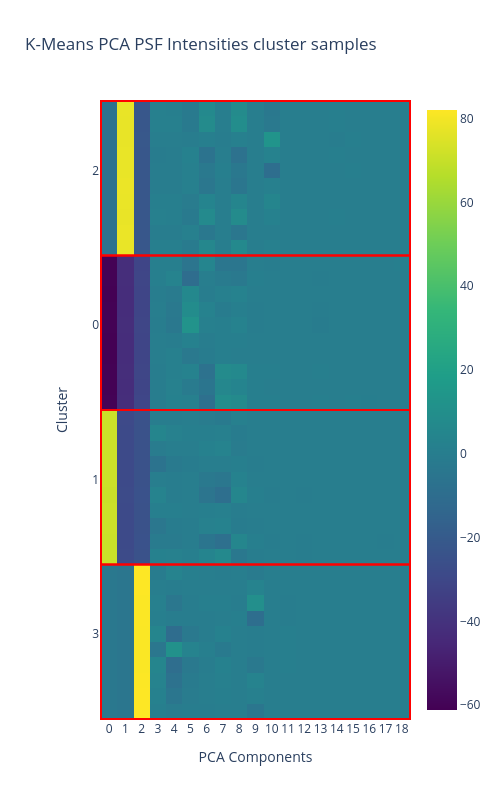
\includegraphics[width=0.4\textwidth]{mdid-pcaintensitiesK-Meansgridclusters.png}}
				\caption{Comparison between original clustering and K-Means clustering from PCA of PSF Intensities}
			\end{figure*}
			\FloatBarrier
			
			\begin{figure*}[ht!]
				\centering
				\subfloat[Original cluster densities from UMAP]{%
					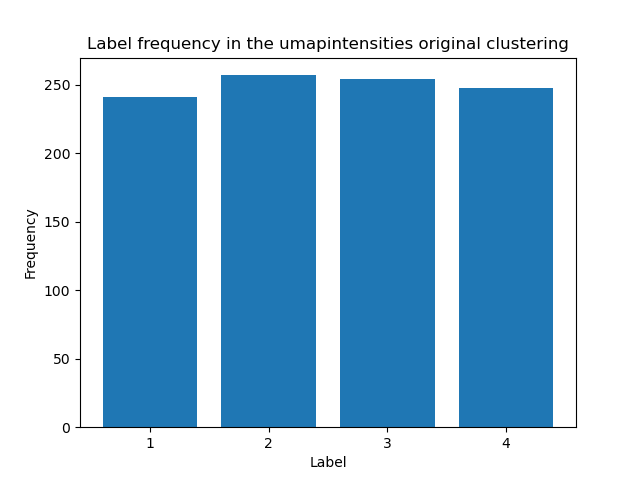
\includegraphics[width=0.45\textwidth]{mdid-umapintensitiesoriginaldensity.png}}
				\hspace{\fill}
				\subfloat[K-Means clusters densities from UMAP]{%
					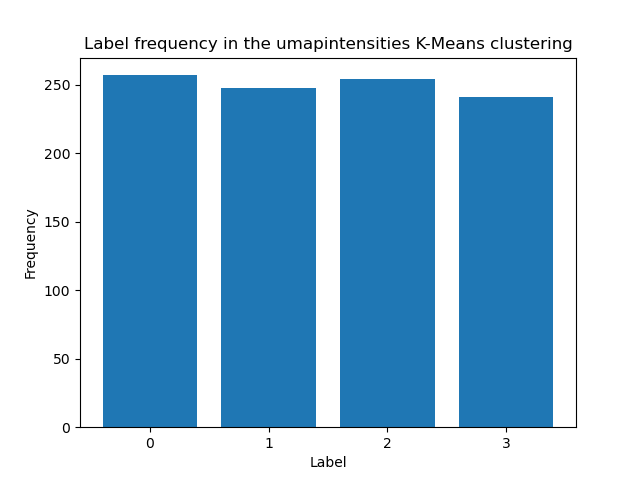
\includegraphics[width=0.45\textwidth]{mdid-umapintensitiesK-Meansdensity.png}}\\
				\subfloat[Original clusters from UMAP]{%
					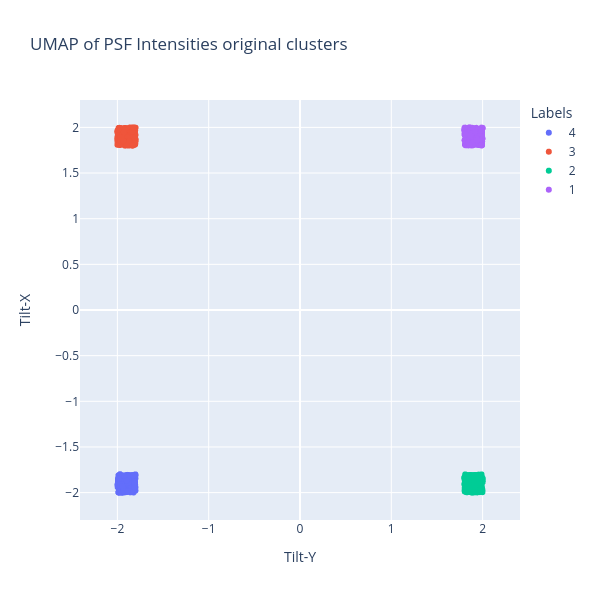
\includegraphics[width=0.45\textwidth]{mdid-umapintensitiesoriginalclusters.png}}
				\hspace{\fill}
				\subfloat[K-Means clusters from UMAP]{%
					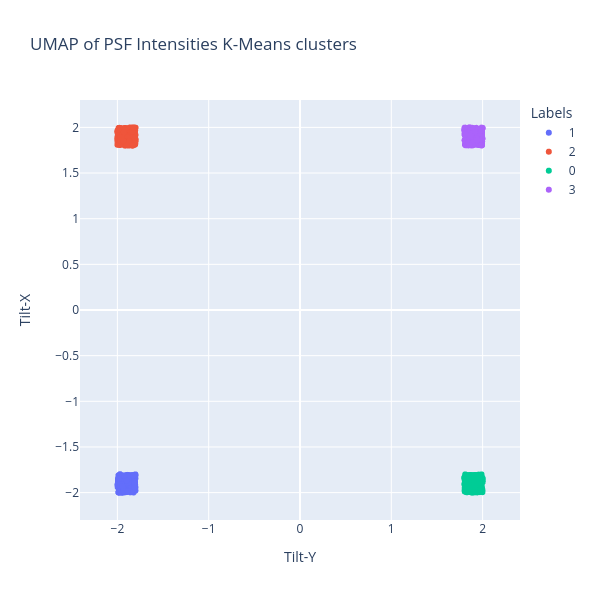
\includegraphics[width=0.45\textwidth]{mdid-umapintensitiesK-Meansclusters.png}}\\
					
				\subfloat[Original cluster samples from UMAP]{%
					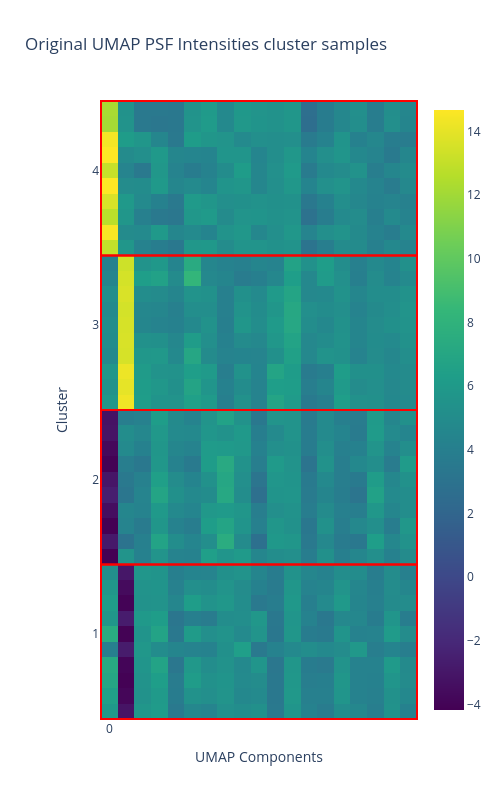
\includegraphics[width=0.4\textwidth]{mdid-umapintensitiesoriginalgridclusters.png}}
				\hspace{\fill}
				\subfloat[K-Means cluster samples from UMAP]{%
					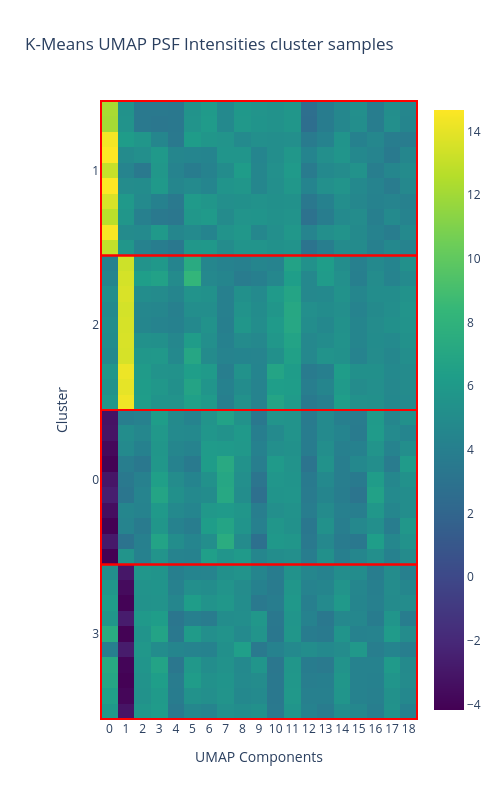
\includegraphics[width=0.4\textwidth]{mdid-umapintensitiesK-Meansgridclusters.png}}
				\caption{Comparison between original clustering and K-Means clustering from UMAP of PSF Intensities}
			\end{figure*}
			\FloatBarrier
		
		\subsubsection{DBSCAN}
			
			A configuration that outputs 4 clusters is searched
			
			\begin{table}[h!]
				\centering
				\begin{tabular}{|c|c|c|}
					\hline
					& \textbf{Number of neighbours} & \textbf{Epsilon}\\
					\hline
					PCA PSF Intensities & 15 & 4.5\\
					\hline
					UMAP PSF Intensities & 10 & 0.85\\
					\hline
				\end{tabular}
				\caption{DBSCAN hyperparameter configuration for PSF Intensities clustering}
			\end{table}
		
			The results are the following:
			
			\begin{figure*}[ht!]
				\centering
				\subfloat[Original cluster densities from PCA]{%
					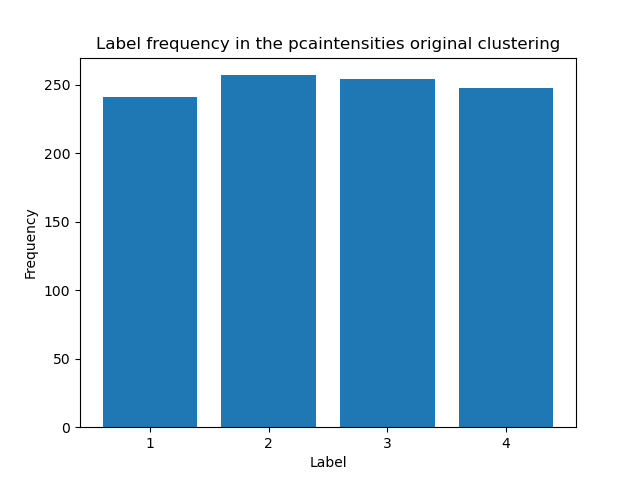
\includegraphics[width=0.45\textwidth]{mdid-pcaintensitiesoriginaldensity.png}}
				\hspace{\fill}
				\subfloat[DBSCAN clusters densities from PCA]{%
					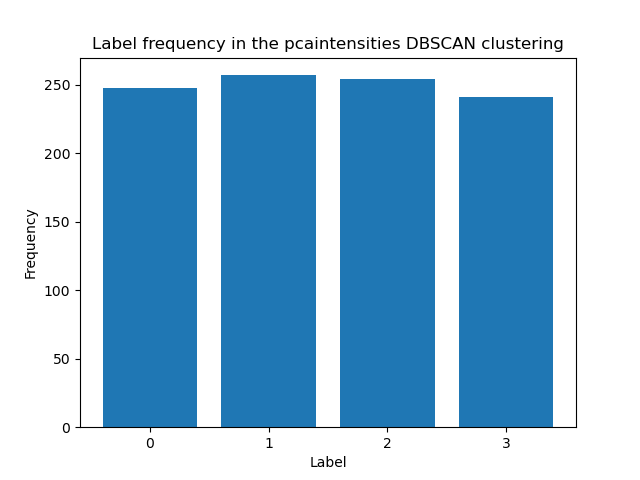
\includegraphics[width=0.45\textwidth]{mdid-pcaintensitiesDBSCANdensity.png}}
				\\
				\subfloat[Original clusters from PCA]{%
					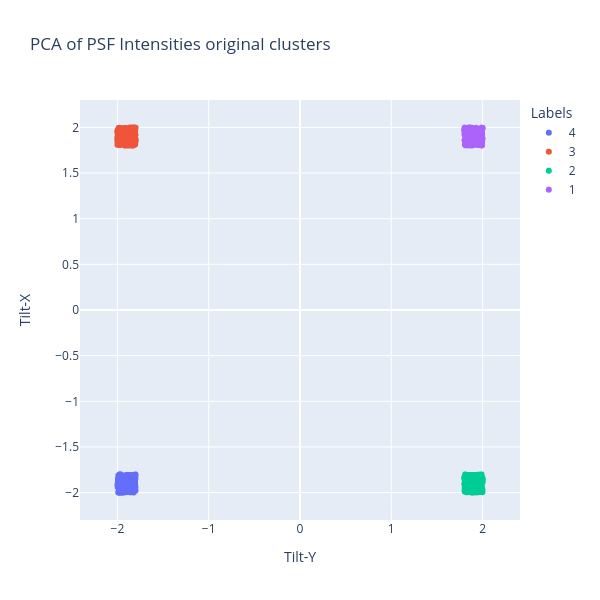
\includegraphics[width=0.45\textwidth]{mdid-pcaintensitiesoriginalclusters.png}}
				\hspace{\fill}
				\subfloat[DBSCAN clusters from PCA]{%
					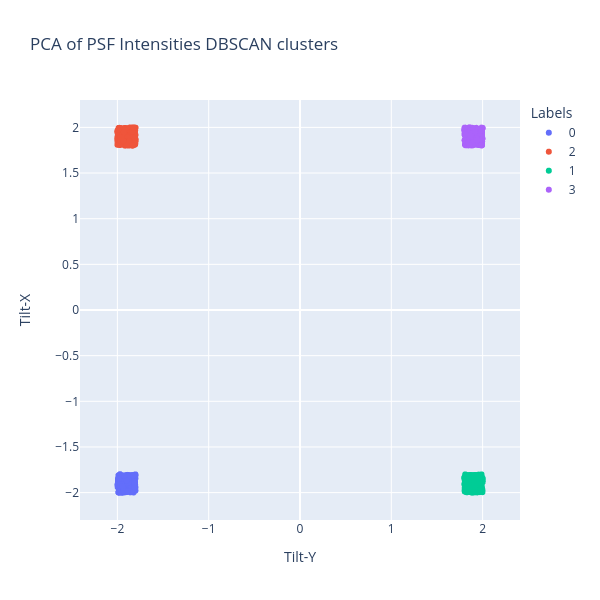
\includegraphics[width=0.45\textwidth]{mdid-pcaintensitiesDBSCANclusters.png}}\\
					
				\subfloat[Original cluster samples from PCA]{%
					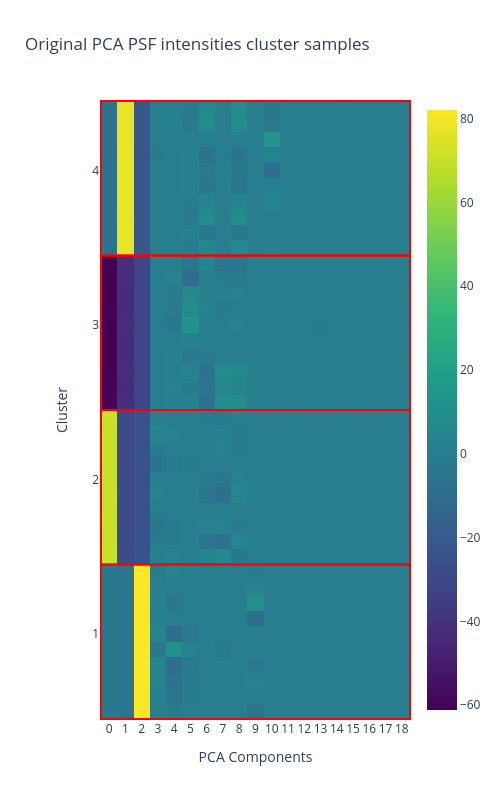
\includegraphics[width=0.4\textwidth]{mdid-pcaintensitiesoriginalgridclusters.png}}
				\hspace{\fill}
				\subfloat[DBSCAN cluster samples from PCA]{%
					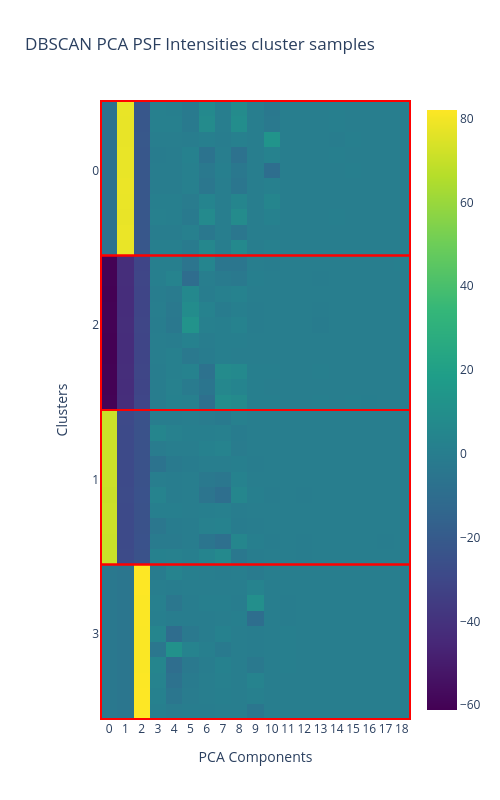
\includegraphics[width=0.4\textwidth]{mdid-pcaintensitiesDBSCANgridclusters.png}}
				\caption{Comparison between original clustering and DBSCAN clustering from PCA of PSF Intensities}
			\end{figure*}
			\FloatBarrier
			
			\begin{figure*}[ht!]
				\centering
				\subfloat[Original cluster densities from UMAP]{%
					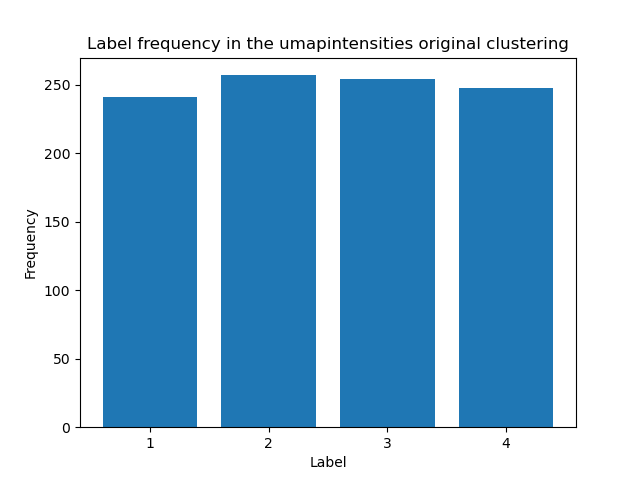
\includegraphics[width=0.45\textwidth]{mdid-umapintensitiesoriginaldensity.png}}
				\hspace{\fill}
				\subfloat[DBSCAN clusters densities from UMAP]{%
					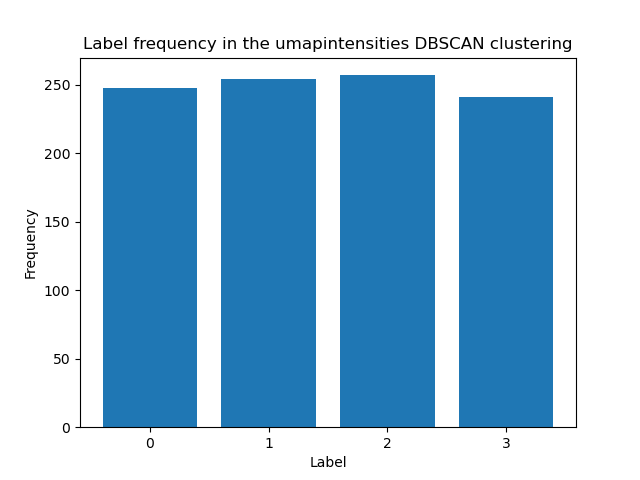
\includegraphics[width=0.45\textwidth]{mdid-umapintensitiesDBSCANdensity.png}}\\
				\subfloat[Original clusters from UMAP]{%
					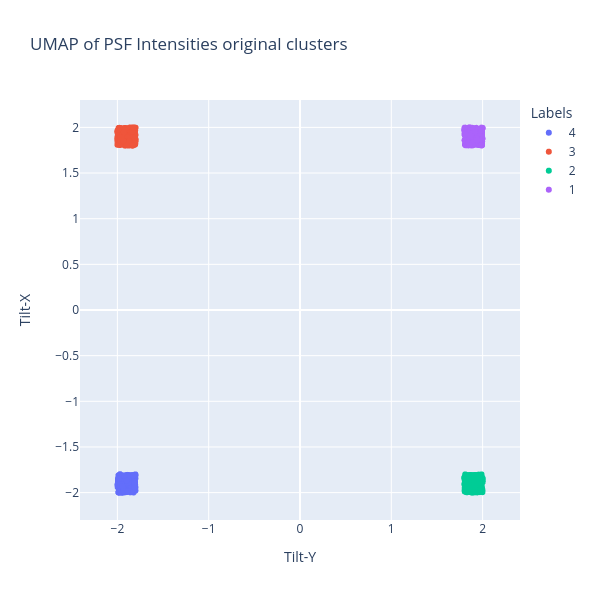
\includegraphics[width=0.45\textwidth]{mdid-umapintensitiesoriginalclusters.png}}
				\hspace{\fill}
				\subfloat[DBSCAN clusters from UMAP]{%
					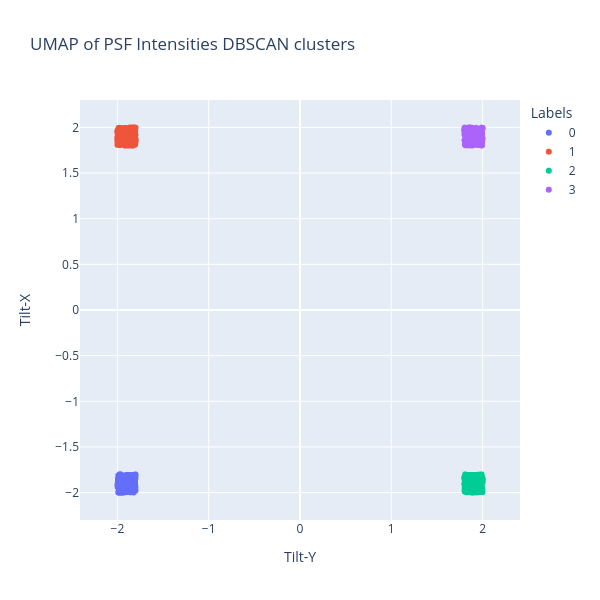
\includegraphics[width=0.45\textwidth]{mdid-umapintensitiesDBSCANclusters.png}}\\
					
				\subfloat[Original cluster samples from UMAP]{%
					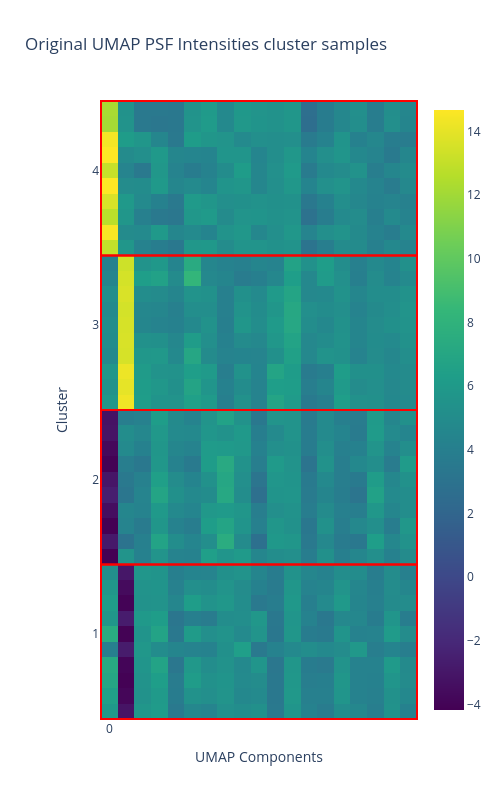
\includegraphics[width=0.4\textwidth]{mdid-umapintensitiesoriginalgridclusters.png}}
				\hspace{\fill}
				\subfloat[DBSCAN cluster samples from UMAP]{%
					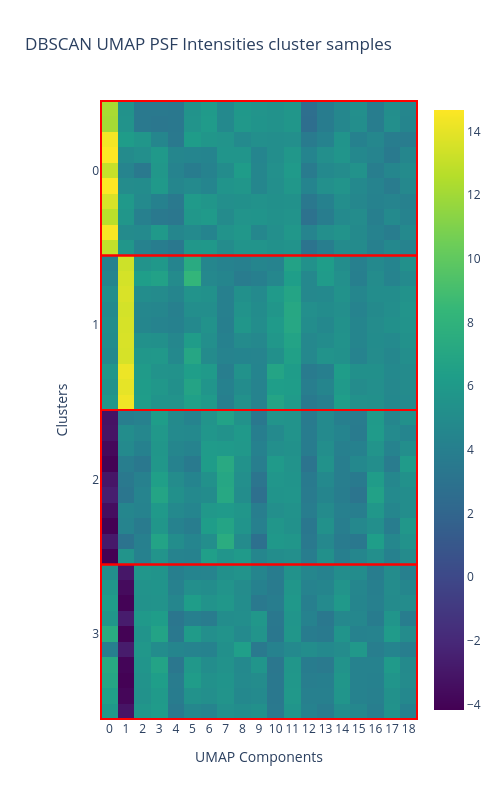
\includegraphics[width=0.4\textwidth]{mdid-umapintensitiesDBSCANgridclusters.png}}
				\caption{Comparison between original clustering and DBSCAN clustering from UMAP of PSF Intensities}
			\end{figure*}
			\FloatBarrier
		
		\subsubsection{HDBSCAN}
			
			A configuration that outputs 4 clusters is searched.
			
			\begin{table}[h!]
				\centering
				\begin{tabular}{|c|c|c|}
					\hline
					& \textbf{Minimum cluster size} \\
					\hline
					PCA PSF Intensities & 21 \\
					\hline
					UMAP PSF Intensities & 25 \\
					\hline
				\end{tabular}
				\caption{HDBSCAN hyperparameter configuration for PSF Intensities clustering}
			\end{table}
			\FloatBarrier
			
			The results are the following:
			
			\begin{figure*}[ht!]
				\centering
				\subfloat[Original cluster densities from PCA]{%
					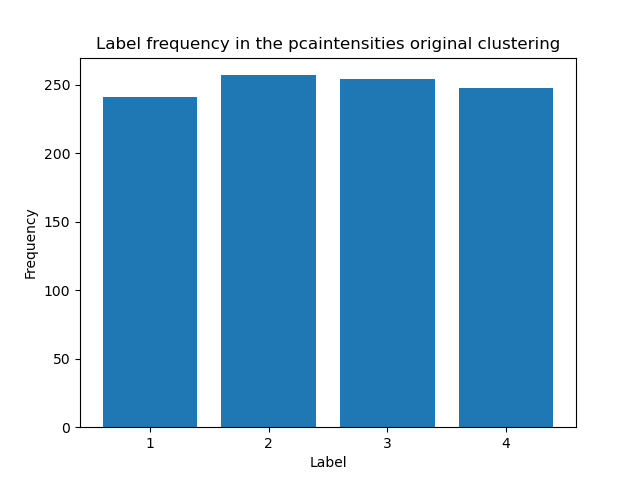
\includegraphics[width=0.45\textwidth]{mdid-pcaintensitiesoriginaldensity.png}}
				\hspace{\fill}
				\subfloat[HDBSCAN clusters densities from PCA]{%
					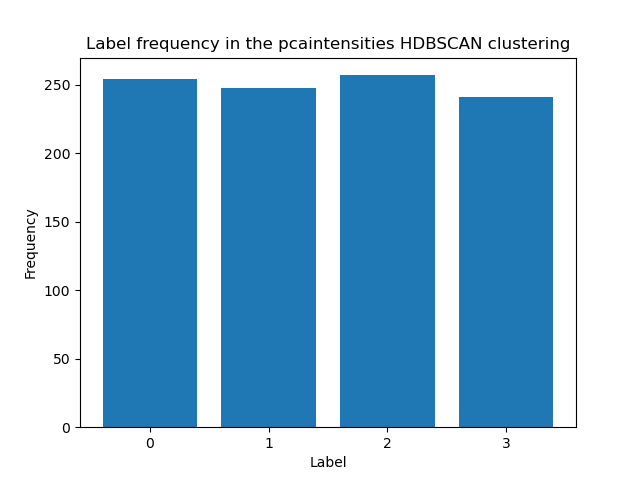
\includegraphics[width=0.45\textwidth]{mdid-pcaintensitiesHDBSCANdensity.png}}
				\\
				\subfloat[Original clusters from PCA]{%
					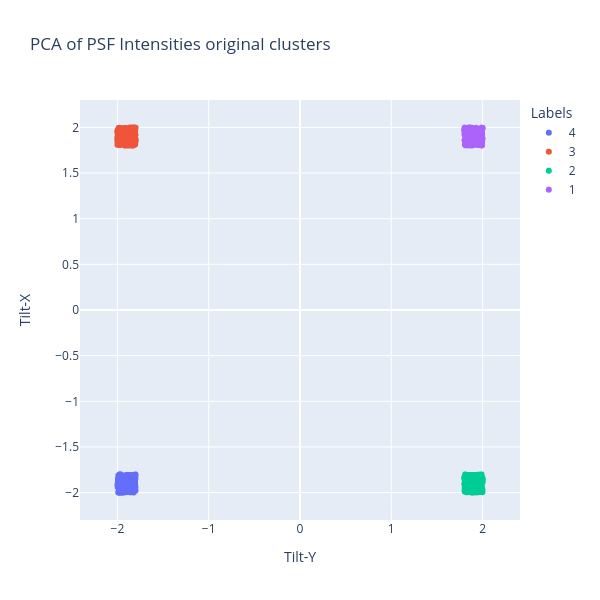
\includegraphics[width=0.45\textwidth]{mdid-pcaintensitiesoriginalclusters.png}}
				\hspace{\fill}
				\subfloat[HDBSCAN clusters from PCA]{%
					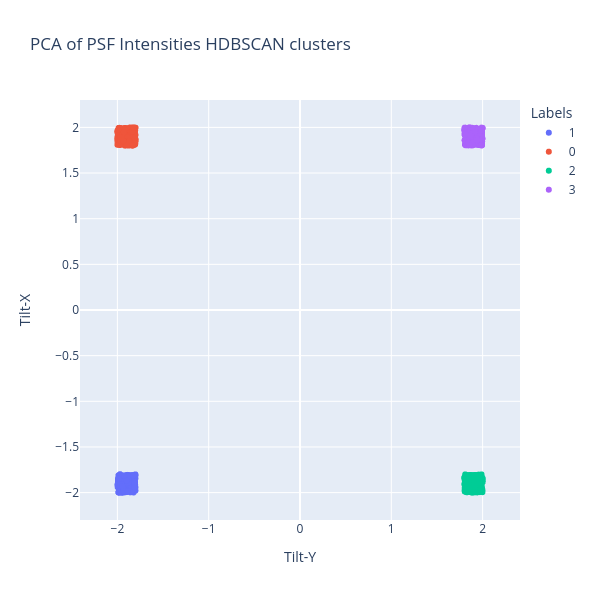
\includegraphics[width=0.45\textwidth]{mdid-pcaintensitiesHDBSCANclusters.png}}\\
					
				\subfloat[Original cluster samples from PCA]{%
					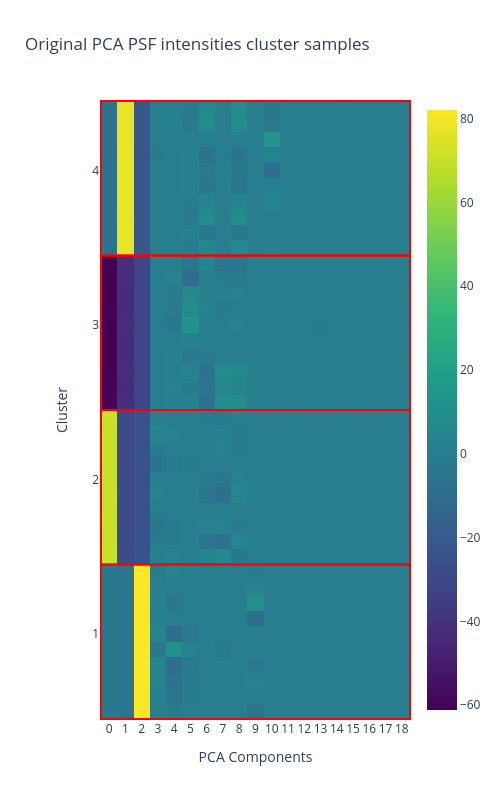
\includegraphics[width=0.4\textwidth]{mdid-pcaintensitiesoriginalgridclusters.png}}
				\hspace{\fill}
				\subfloat[HDBSCAN cluster samples from PCA]{%
					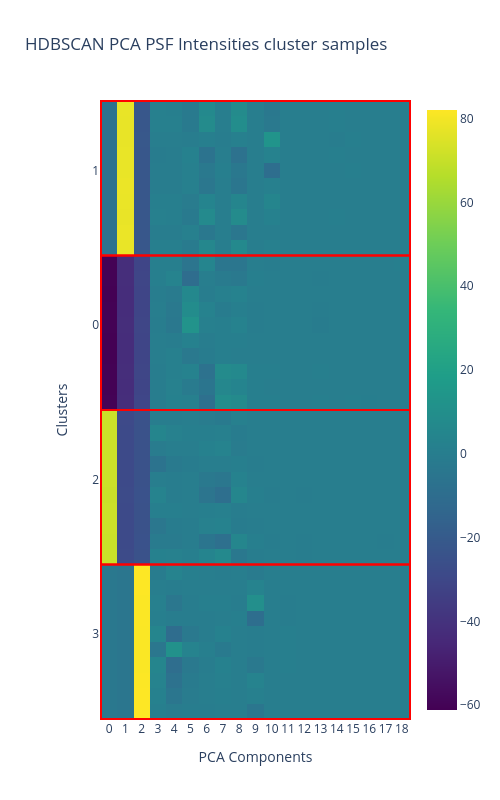
\includegraphics[width=0.4\textwidth]{mdid-pcaintensitiesHDBSCANgridclusters.png}}
				\caption{Comparison between original clustering and HDBSCAN clustering from PCA of PSF Intensities}
			\end{figure*}
			\FloatBarrier
			
			\begin{figure*}[ht!]
				\centering
				\subfloat[Original cluster densities from UMAP]{%
					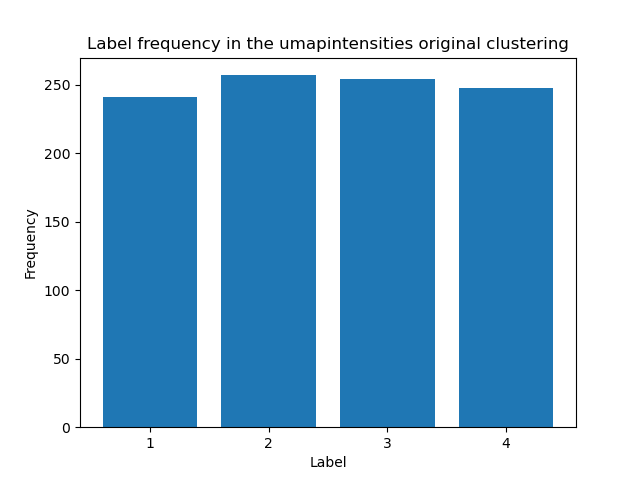
\includegraphics[width=0.45\textwidth]{mdid-umapintensitiesoriginaldensity.png}}
				\hspace{\fill}
				\subfloat[HDBSCAN clusters densities from UMAP]{%
					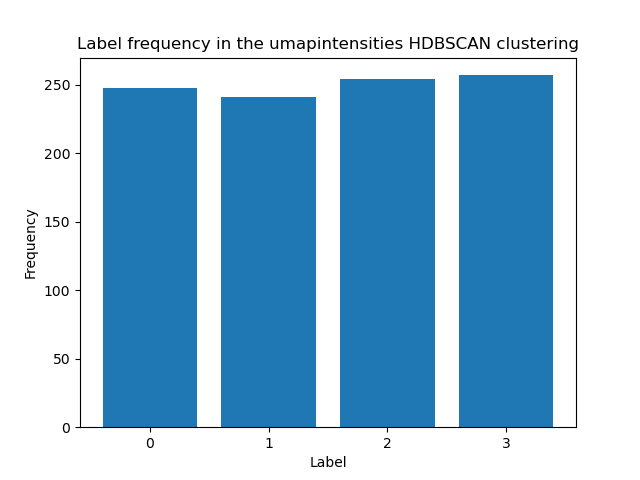
\includegraphics[width=0.45\textwidth]{mdid-umapintensitiesHDBSCANdensity.png}}\\
				\subfloat[Original clusters from UMAP]{%
					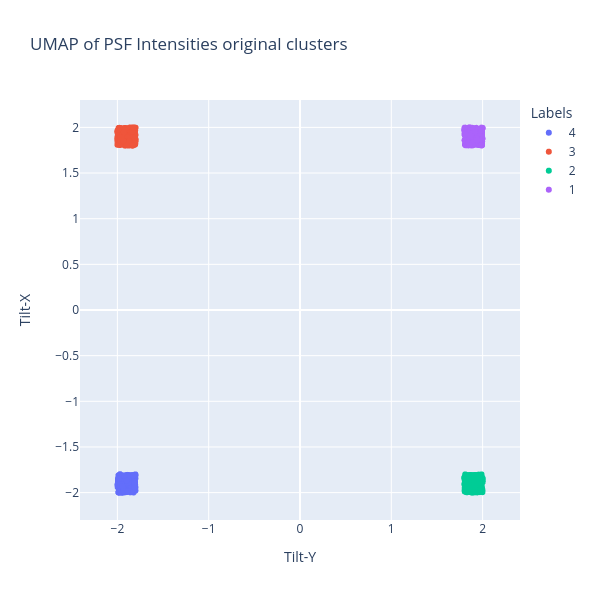
\includegraphics[width=0.45\textwidth]{mdid-umapintensitiesoriginalclusters.png}}
				\hspace{\fill}
				\subfloat[HDBSCAN clusters from UMAP]{%
					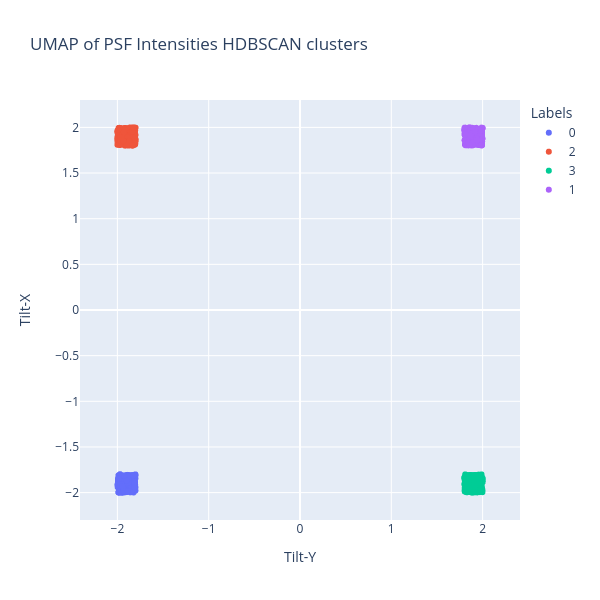
\includegraphics[width=0.45\textwidth]{mdid-umapintensitiesHDBSCANclusters.png}}\\
					
				\subfloat[Original cluster samples from UMAP]{%
					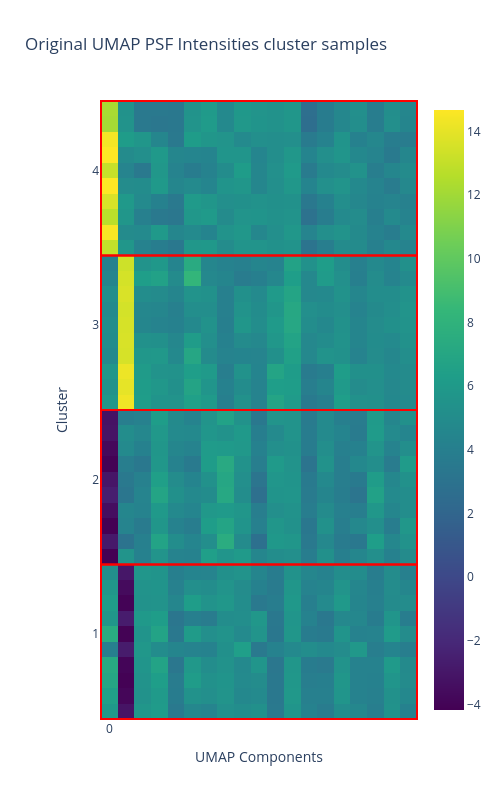
\includegraphics[width=0.4\textwidth]{mdid-umapintensitiesoriginalgridclusters.png}}
				\hspace{\fill}
				\subfloat[HDBSCAN cluster samples from UMAP]{%
					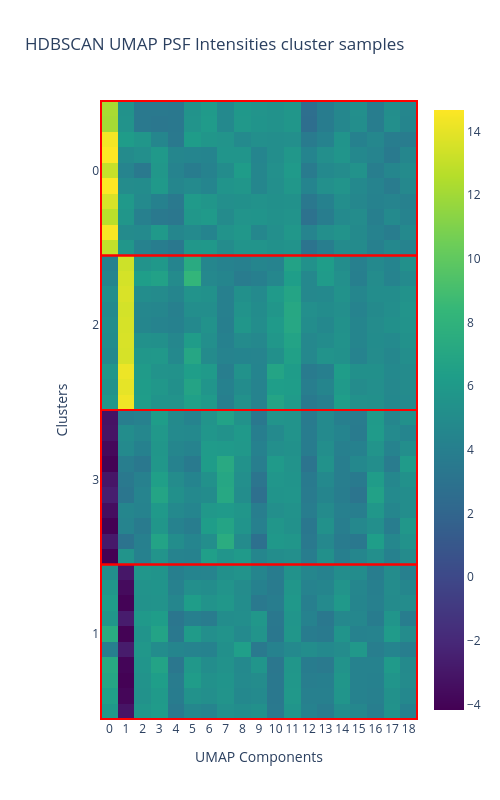
\includegraphics[width=0.4\textwidth]{mdid-umapintensitiesHDBSCANgridclusters.png}}
				\caption{Comparison between original clustering and HDBSCAN clustering from UMAP of PSF Intensities}
			\end{figure*}
			\FloatBarrier
		
		\subsubsection{Agglomerative clustering}
			\begin{table}[h!]
				\centering
				\begin{tabular}{|c|c|}
					\hline
					 & \textbf{Number of clusters} \\
					\hline
					PCA PSF Intensities & 4 \\
					\hline
					UMAP PSF Intensities & 4 \\
					\hline
				\end{tabular}
				\caption{Agglomerative hyperparameter configuration for PSF Intensities clustering}
			\end{table}
			\FloatBarrier
			The results are the following:
			
			\begin{figure*}[ht!]
				\centering
				\subfloat[Original cluster densities from PCA]{%
					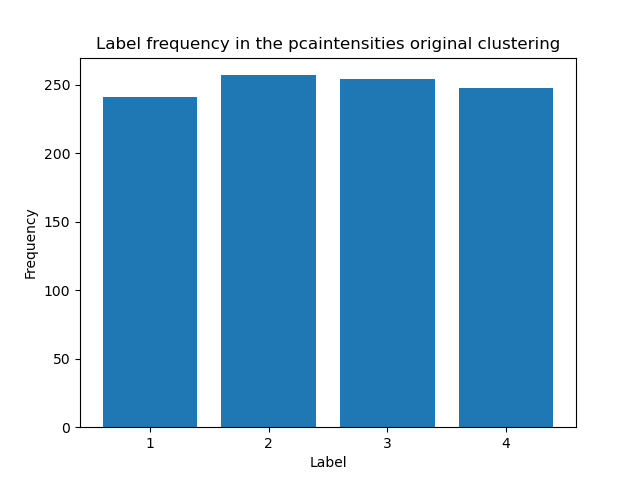
\includegraphics[width=0.45\textwidth]{mdid-pcaintensitiesoriginaldensity.png}}
				\hspace{\fill}
				\subfloat[Agglomerative clusters densities from PCA]{%
					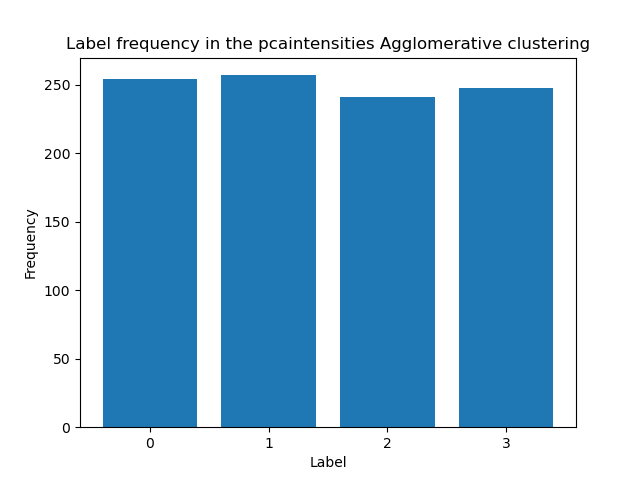
\includegraphics[width=0.45\textwidth]{mdid-pcaintensitiesAgglomerativedensity.png}}
				\\
				\subfloat[Original clusters from PCA]{%
					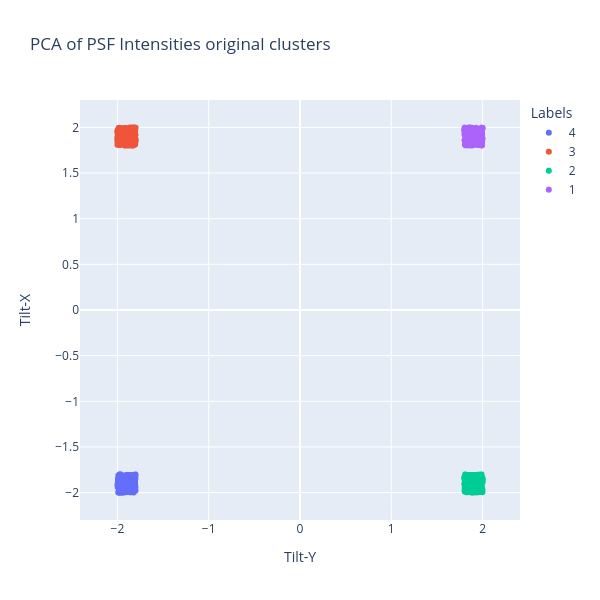
\includegraphics[width=0.45\textwidth]{mdid-pcaintensitiesoriginalclusters.png}}
				\hspace{\fill}
				\subfloat[Agglomerative clusters from PCA]{%
					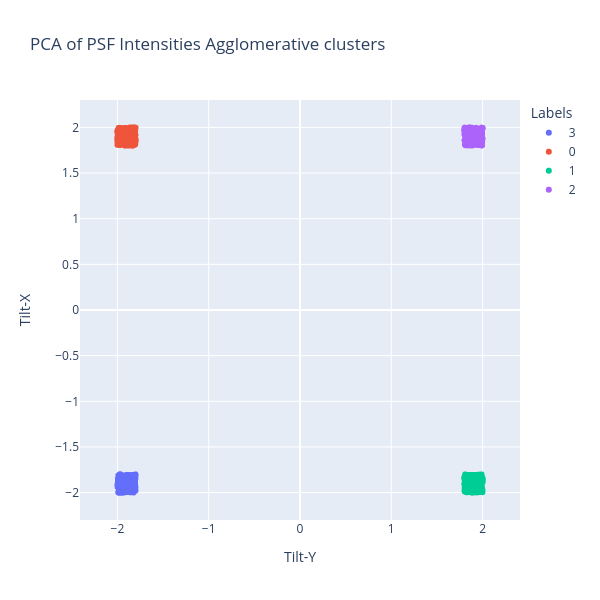
\includegraphics[width=0.45\textwidth]{mdid-pcaintensitiesAgglomerativeclusters.png}}\\
					
				\subfloat[Original cluster samples from PCA]{%
					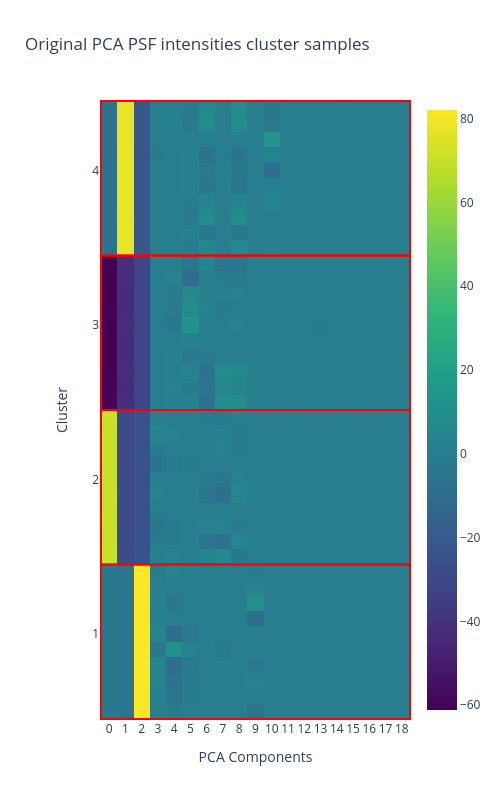
\includegraphics[width=0.4\textwidth]{mdid-pcaintensitiesoriginalgridclusters.png}}
				\hspace{\fill}
				\subfloat[Agglomerative cluster samples from PCA]{%
					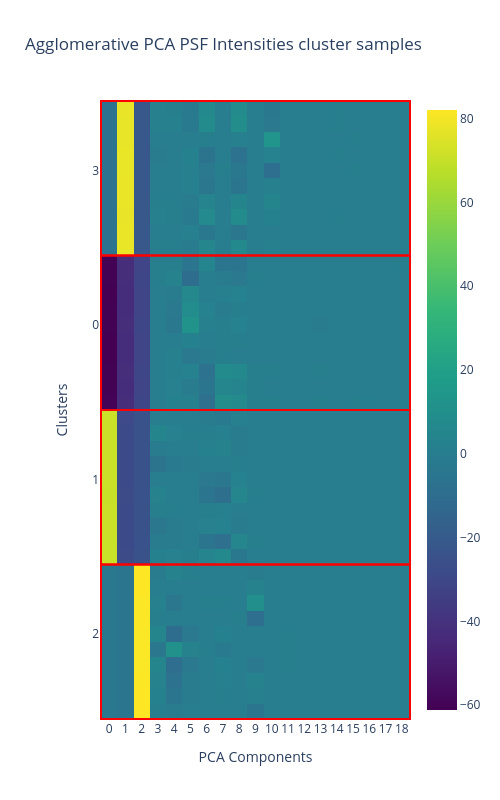
\includegraphics[width=0.4\textwidth]{mdid-pcaintensitiesAgglomerativegridclusters.png}}
				\caption{Comparison between original clustering and Agglomerative clustering}
			\end{figure*}
			\FloatBarrier
			
			\begin{figure*}[ht!]
				\centering
				\subfloat[Original cluster densities from UMAP]{%
					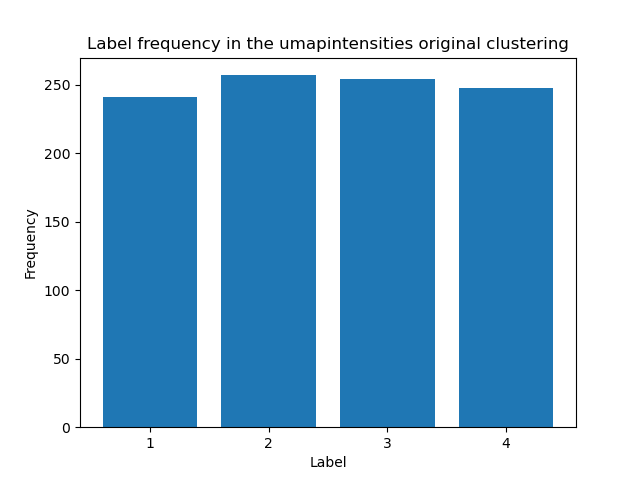
\includegraphics[width=0.45\textwidth]{mdid-umapintensitiesoriginaldensity.png}}
				\hspace{\fill}
				\subfloat[Agglomerative clusters densities from UMAP]{%
					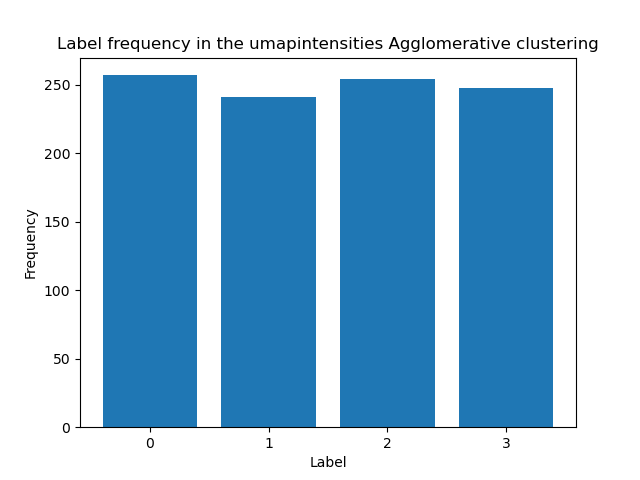
\includegraphics[width=0.45\textwidth]{mdid-umapintensitiesAgglomerativedensity.png}}\\
				\subfloat[Original clusters from UMAP]{%
					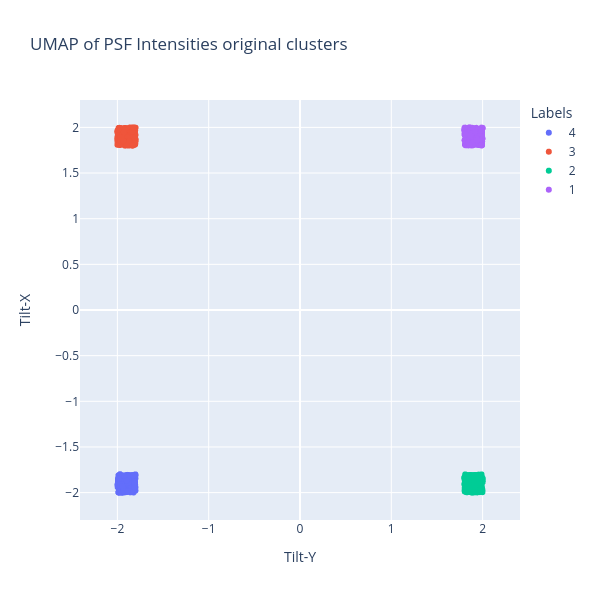
\includegraphics[width=0.45\textwidth]{mdid-umapintensitiesoriginalclusters.png}}
				\hspace{\fill}
				\subfloat[Agglomerative clusters from UMAP]{%
					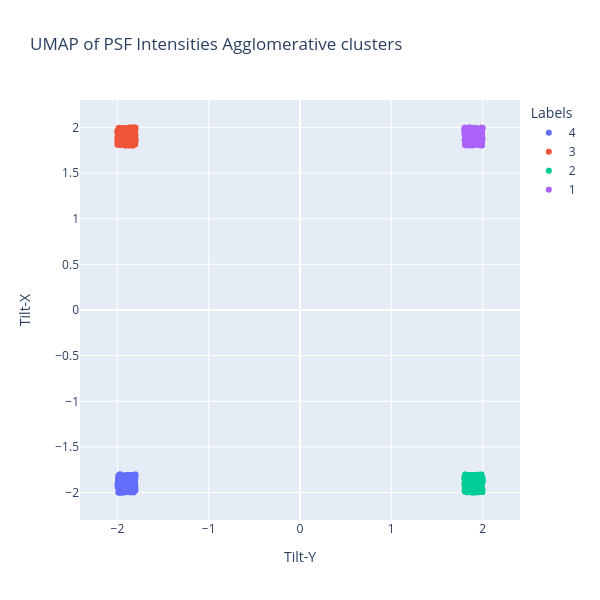
\includegraphics[width=0.45\textwidth]{mdid-umapintensitiesAgglomerativeclusters.png}}\\
					
				\subfloat[Original cluster samples from UMAP]{%
					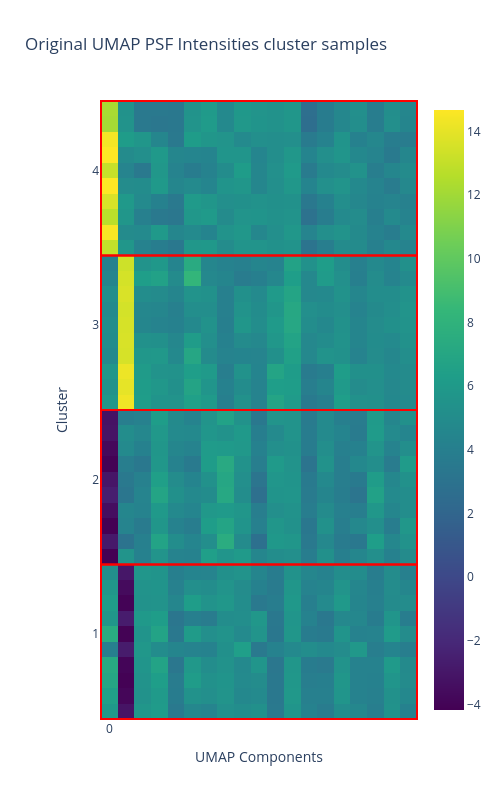
\includegraphics[width=0.4\textwidth]{mdid-umapintensitiesoriginalgridclusters.png}}
				\hspace{\fill}
				\subfloat[Agglomerative cluster samples from UMAP]{%
					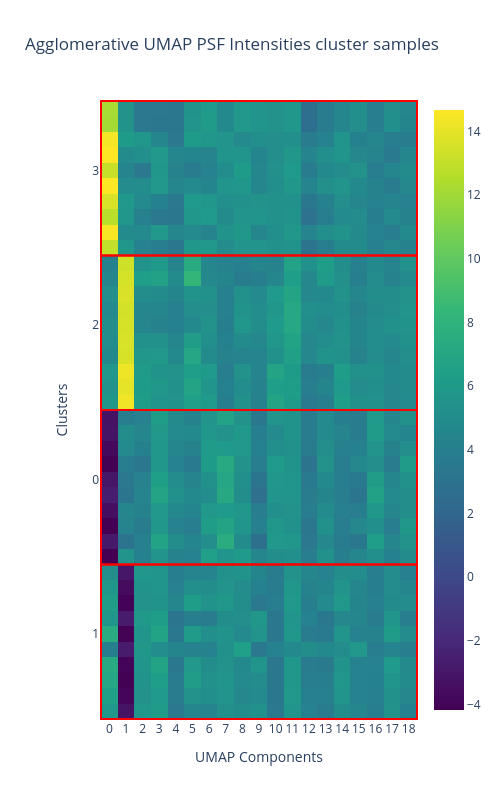
\includegraphics[width=0.4\textwidth]{mdid-umapintensitiesAgglomerativegridclusters.png}}
				\caption{Comparison between original clustering and Agglomerative clustering from UMAP of PSF Intensities}
			\end{figure*}
			\FloatBarrier
		
		\subsubsection{Summary}
		
		\begin{figure*}[ht!]
				\centering
				\subfloat[Original cluster densities from PCA]{%
					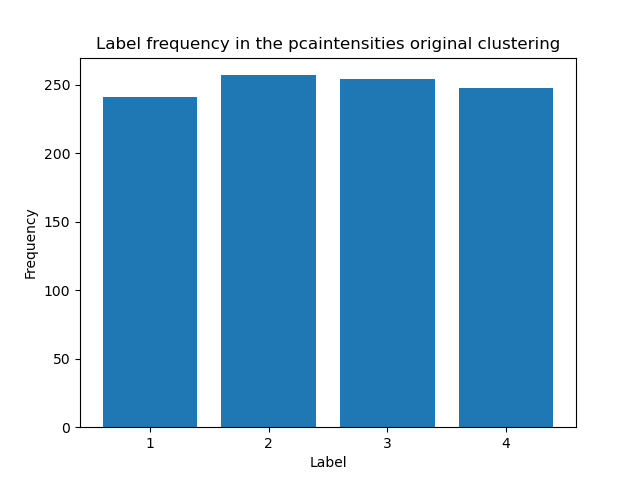
\includegraphics[width=0.18\textwidth]{mdid-pcaintensitiesoriginaldensity.png}}
				\hspace{\fill}
				\subfloat[K-means cluster densities from PCA]{%
					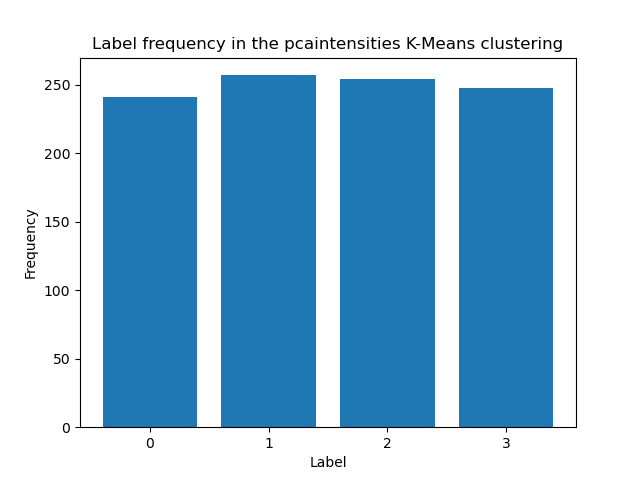
\includegraphics[width=0.18\textwidth]{mdid-pcaintensitiesK-Meansdensity.png}}
				\hspace{\fill}
				\subfloat[DBSCAN cluster densities from PCA]{%
					\includegraphics[width=0.18\textwidth]{mdid-pcaintensitiesDBSCANdensity.png}}
				\hspace{\fill}
				\subfloat[HDBSCAN cluster densities from PCA]{%
					\includegraphics[width=0.18\textwidth]{mdid-pcaintensitiesHDBSCANdensity.png}}
				\hspace{\fill}
				\subfloat[Agglomerative cluster densities from PCA]{%
					\includegraphics[width=0.18\textwidth]{mdid-pcaintensitiesAgglomerativedensity.png}}
				\\
				
				\subfloat[Original cluster from PCA]{%
					\includegraphics[width=0.18\textwidth]{mdid-pcaintensitiesoriginalclusters.png}}
				\hspace{\fill}
				\subfloat[K-means clusters from PCA]{%
					\includegraphics[width=0.18\textwidth]{mdid-pcaintensitiesK-Meansclusters.png}}
				\hspace{\fill}
				\subfloat[DBSCAN cluster clusters from PCA]{%
					\includegraphics[width=0.18\textwidth]{mdid-pcaintensitiesDBSCANclusters.png}}
				\hspace{\fill}
				\subfloat[HDBSCAN clusters from PCA]{%
					\includegraphics[width=0.18\textwidth]{mdid-pcaintensitiesHDBSCANclusters.png}}
				\hspace{\fill}
				\subfloat[Agglomerative clusters from PCA]{%
					\includegraphics[width=0.18\textwidth]{mdid-pcaintensitiesAgglomerativeclusters.png}}\\
				
				\subfloat[Original cluster samples from PCA]{%
					\includegraphics[width=0.18\textwidth]{mdid-pcaintensitiesoriginalgridclusters.png}}
				\hspace{\fill}
				\subfloat[K-means cluster samples from PCA]{%
					\includegraphics[width=0.18\textwidth]{mdid-pcaintensitiesK-Meansgridclusters.png}}
				\hspace{\fill}
				\subfloat[DBSCAN cluster samplesfrom PCA]{%
					\includegraphics[width=0.18\textwidth]{mdid-pcaintensitiesDBSCANgridclusters.png}}
				\hspace{\fill}
				\subfloat[HDBSCAN cluster samples from PCA]{%
					\includegraphics[width=0.18\textwidth]{mdid-pcaintensitiesHDBSCANgridclusters.png}}
				\hspace{\fill}
				\subfloat[Agglomerative cluster samples from PCA]{%
					\includegraphics[width=0.18\textwidth]{mdid-pcaintensitiesAgglomerativegridclusters.png}}
				
				\caption{Comparison between clustering PCA PSF Intensities algorithms}
			\end{figure*}
		\FloatBarrier
		
		\begin{table}[h!]
    			\centering
    			\begin{tabular}{|c|c|c|c|c|c|}
        			\hline
        			& \textbf{Original} & \textbf{K-Means} & \textbf{DBSCAN} & \textbf{HDBSCAN} & \textbf{Agglomerative} \\
        			\hline
        			\textbf{Original} & \diagbox{}{} & 1 & 1 & 1 & 1 \\
       			\hline
        			\textbf{K-Means} &  & \diagbox{}{} & 1 & 1 & 1\\
        			\hline
        			\textbf{DBSCAN} &  &  & \diagbox{}{} & 1 & 1\\
        			\hline
        			\textbf{HDBSCAN} &  &  &  & \diagbox{}{} & 1\\
       			\hline
    			\end{tabular}
    			\caption{Normalized Mutual Information between PCA PSF Intensities clusters}
		\end{table}
		
		\begin{figure*}[ht!]
				\centering
				\subfloat[Original cluster densities from UMAP]{%
					\includegraphics[width=0.18\textwidth]{mdid-umapintensitiesoriginaldensity.png}}
				\hspace{\fill}
				\subfloat[K-means cluster densities from UMAP]{%
					\includegraphics[width=0.18\textwidth]{mdid-umapintensitiesK-Meansdensity.png}}
				\hspace{\fill}
				\subfloat[DBSCAN cluster densities from UMAP]{%
					\includegraphics[width=0.18\textwidth]{mdid-umapintensitiesDBSCANdensity.png}}
				\hspace{\fill}
				\subfloat[HDBSCAN cluster densities from UMAP]{%
					\includegraphics[width=0.18\textwidth]{mdid-umapintensitiesHDBSCANdensity.png}}
				\hspace{\fill}
				\subfloat[Agglomerative cluster densities from UMAP]{%
					\includegraphics[width=0.18\textwidth]{mdid-umapintensitiesAgglomerativedensity.png}}
				\\
				
				\subfloat[Original cluster from UMAP]{%
					\includegraphics[width=0.18\textwidth]{mdid-umapintensitiesoriginalclusters.png}}
				\hspace{\fill}
				\subfloat[K-means clusters from UMAP]{%
					\includegraphics[width=0.18\textwidth]{mdid-umapintensitiesK-Meansclusters.png}}
				\hspace{\fill}
				\subfloat[DBSCAN cluster clusters from UMAP]{%
					\includegraphics[width=0.18\textwidth]{mdid-umapintensitiesDBSCANclusters.png}}
				\hspace{\fill}
				\subfloat[HDBSCAN clusters from UMAP]{%
					\includegraphics[width=0.18\textwidth]{mdid-umapintensitiesHDBSCANclusters.png}}
				\hspace{\fill}
				\subfloat[Agglomerative clusters from UMAP]{%
					\includegraphics[width=0.18\textwidth]{mdid-umapintensitiesAgglomerativeclusters.png}}\\
				
				\subfloat[Original cluster samples from UMAP]{%
					\includegraphics[width=0.18\textwidth]{mdid-umapintensitiesoriginalgridclusters.png}}
				\hspace{\fill}
				\subfloat[K-means cluster samples from UMAP]{%
					\includegraphics[width=0.18\textwidth]{mdid-umapintensitiesK-Meansgridclusters.png}}
				\hspace{\fill}
				\subfloat[DBSCAN cluster samplesfrom UMAP]{%
					\includegraphics[width=0.18\textwidth]{mdid-umapintensitiesDBSCANgridclusters.png}}
				\hspace{\fill}
				\subfloat[HDBSCAN cluster samples from UMAP]{%
					\includegraphics[width=0.18\textwidth]{mdid-umapintensitiesHDBSCANgridclusters.png}}
				\hspace{\fill}
				\subfloat[Agglomerative cluster samples from UMAP]{%
					\includegraphics[width=0.18\textwidth]{mdid-umapintensitiesAgglomerativegridclusters.png}}
				
				\caption{Comparison between clustering UMAP PSF Intensities algorithms}
			\end{figure*}
		\FloatBarrier
		
		\begin{table}[h!]
    			\centering
    			\begin{tabular}{|c|c|c|c|c|c|}
        			\hline
        			& \textbf{Original} & \textbf{K-Means} & \textbf{DBSCAN} & \textbf{HDBSCAN} & \textbf{Agglomerative} \\
        			\hline
        			\textbf{Original} & \diagbox{}{} & 1 & 1 & 1 & 1 \\
       			\hline
        			\textbf{K-Means} &  & \diagbox{}{} & 1 & 1 & 1\\
        			\hline
        			\textbf{DBSCAN} &  &  & \diagbox{}{} & 1 & 1\\
        			\hline
        			\textbf{HDBSCAN} &  &  &  & \diagbox{}{} & 1\\
       			\hline
    			\end{tabular}
    			\caption{Normalized Mutual Information between UMAP PSF Intensities clusters}
		\end{table}